
\documentclass[addpoints]{exam}
\usepackage[utf8]{inputenc}
\usepackage{amsmath}
\usepackage{mathtools}
\usepackage{multicol}
\usepackage{tikz}
\usepackage{pgfplots}
\newcommand\Myperm[2][^n]{\prescript{#1\mkern-2.5mu}{}P_{#2}}
	\newcommand\Mycomb[2][^n]{\prescript{#1\mkern-0.5mu}{}C_{#2}}
		\usetikzlibrary{datavisualization}
\usetikzlibrary{datavisualization.formats.functions}
\usepackage{relsize}
\usepackage{dirtytalk}
\usepackage{graphicx}
\graphicspath{ {./drift/} }
\DeclarePairedDelimiter{\ceil}{\lceil}{\rceil}
\usepackage{geometry}
\usepackage{draftwatermark}
\usepackage[banglamainfont=Kalpurush,
            banglattfont=Siyam Rupali
           ]{latexbangla}
\SetWatermarkText{\textit{$fo\phi(x) = f((\phi(x)))$}}
\begin{document}
\begin{center}
\fbox{\fbox{\parbox{5.5in}{\centering  ফাংশন ও লেখচিত্র}}}
\end{center}

\vspace{5mm}

%-------------------------------------------------------------------

%Here, the questions begin
\begin{questions}

%First question below
\question   $ f(x) = \dfrac{-1}{|1-x|} $  ফাংশনের রেঞ্জ (The range of the function $ f(x) = \dfrac{-1}{|1-x|} $ is) \hfill \textsc{DU:2018-19}

\begin{oneparchoices}
\choice $ \mathbb{R}-{1} $
\choice $ \mathbb{R}-{0} $
\choice $ \mathbb{R}-{0,1} $
\choice  $ (-\infty, 0) $

\end{oneparchoices}
\question $\mathlarger{ f(x) = \dfrac{1}{|\sqrt{x}|}, \; g(x)=x^2}$  হলে এর ডোমেন (The domain of  $ f(x) = \dfrac{1}{\sqrt{|x|}} $ is) \hfill \textsc{DU:2017-18}

\begin{oneparchoices}
\choice $ [0,+\infty) $
\choice $ (0,+\infty) $
\choice $ (-\infty, +\infty) $
\choice $ (-\infty, 0)\cup (0, +\infty)  $

\end{oneparchoices}

\question $\mathlarger{ f(x) = \sin x, \; g(x)=x^2}$  হলে  $\mathlarger{f(g(\frac{\sqrt{\pi}}{2}))}$ এর মান \hfill \textsc{DU:2016-17, 09-10}

\begin{oneparchoices}
  \choice $\mathlarger{\frac{\sqrt{2}}{2} }$
 \choice $\mathlarger{\frac{\sqrt{3}}{2} }$
 \choice $\mathlarger{\frac{1}{2} }$
 \choice $\mathlarger{1}$
\end{oneparchoices}
\question $\mathlarger{f:\mathbb{R} \rightarrow \mathbb{R}}$ কে $\mathlarger{f(x)=e^{x-3}}$ দ্বারা সংজ্ঞায়িত করা হলে $\mathlarger{f^{-1}(e)}$ এর মান  \hfill \textsc{DU:2015-16}

\begin{oneparchoices}
 \choice $\mathlarger{4}$
 \choice $\mathlarger{3}$
 \choice $\mathlarger{2}$
 \choice $\mathlarger{0}$
\end{oneparchoices}


\question $\mathlarger{y=\frac{1}{\sqrt{4-x}}}$ ফাংশনের ডোমেন ও রেঞ্জ \hfill \textsc{DU:2015-16}

\begin{oneparchoices}
 \choice $\mathlarger{-\infty<x \le 4;\; 0\le y < \infty}$
 \choice $\mathlarger{-\infty<x < 4;\; 0< y < \infty}$
 \choice $\mathlarger{-\infty<x < 4;\; 0\le y < \infty}$
 \choice $\mathlarger{-\infty<x \le 4;\; 0< y < \infty}$
\end{oneparchoices}

\question $\mathlarger{y=\frac{1}{\sqrt{4-x^{2}}}}$ বাস্তব ফাংশনটির ডোমেন ও রেঞ্জ \hfill \textsc{DU:2014-15}

\begin{oneparchoices}
 \choice $\mathlarger{x<2;\; y>\frac{1}{2}}$
 \choice $\mathlarger{-2<x < 2;\; y \ge \frac{1}{2}}$
\choice $\mathlarger{-2 \le x \le 2;\; y < \frac{1}{2}}$
 \choice $\mathlarger{-x< -2\;\& \;  x>2;\; -2< y < 2}$
\end{oneparchoices}

\question $\mathlarger{f(x)=\sqrt{x^{2}-5x+6}}$ ফাংশনের ডোমেন ও রেঞ্জ    \hfill \textsc{DU:2013-14}

\begin{oneparchoices}
 \choice $\mathlarger{x \le 2,\; 3\le x\;\text{and}\; y \ge 0}$
 \choice $\mathlarger{2\le x \le 3\;\text{and}\;  y \ge 0}$
 \choice $\mathlarger{ x \ge 3\;\text{and}\;  y \ge 0}$
 \choice $\mathlarger{x \le 2,\; x\ge 3\;\text{and}\; y \ge 0}$
\end{oneparchoices}

\question যদি $\mathlarger{f(x)=(x-2)(1-x)}$ হয় তবে $\mathlarger{f(f(3))}$এর মান  \hfill \textsc{DU:2013-14}

\begin{oneparchoices}
 \choice $\mathlarger{12}$
 \choice $\mathlarger{9}$
 \choice $\mathlarger{ -12}$
 \choice $\mathlarger{8}$
\end{oneparchoices}

\question $\mathlarger{f(x)=4-(x-3)^{2}}$ ফাংশনের ডোমেন ও রেঞ্জ \hfill \textsc{DU:2012-13}

\begin{oneparchoices}
 \choice $\mathlarger{\mathbb{R},\; \mathbb{R} }$
 \hspace*{1.5cm}\choice $\mathlarger{\mathbb{R},\; x\le 4}$
 \choice $x\ge 4,\; \mathlarger{\mathbb{R}}$
 \hspace*{.93cm}\choice $\mathlarger{\mathbb{R},\; x\ge 4}$
\end{oneparchoices}

\question যদি $\mathlarger{f(x)=\frac{x-3}{2x+1}}$ এবং $\mathlarger{x \neq \frac{1}{2}}$ হয় তবে $\mathlarger{f^{-1}(-2)}$  এর মান   \hfill \textsc{DU:2012-13,08-09}

\begin{oneparchoices}
 \choice $\mathlarger{\frac{1}{5} }$
 \choice $\mathlarger{\frac{1}{2}}$
 \choice $\mathlarger{2}$
 \choice $\mathlarger{5}$
\end{oneparchoices}

\question $\mathlarger{x^{2}-2x+5}$ এর নূন্যতম মান   \hfill \textsc{DU:2011-12}

\begin{oneparchoices}
 \choice $\mathlarger{1 }$
 \choice $\mathlarger{2}$
 \choice $\mathlarger{3}$
 \choice $\mathlarger{4}$
\end{oneparchoices}

\question $\mathlarger{f(x) = 3x^{3}+3}$ এবং $\mathlarger{g(x)=\sqrt[3]{\frac{x-2}{3}}}$ হয় তবে  $\mathlarger{(f \circ g)(3)}$ এর মান  \hfill \textsc{DU:2011-12}

\begin{oneparchoices}
 \choice $\mathlarger{1 }$
 \choice $\mathlarger{2}$
 \choice $\mathlarger{3}$
 \choice $\mathlarger{4}$
\end{oneparchoices}

\question $\mathlarger{5-3x-x^{2}}$ এর সর্বোচ্চ মান  \hfill \textsc{DU:2010-11}

\begin{oneparchoices}
 \choice $\mathlarger{1 }$
 \choice $\mathlarger{2}$
 \choice $\mathlarger{3}$
 \choice $\mathlarger{4}$
\end{oneparchoices}

\question $ f(x) = \dfrac{5x+3}{4x-5}$ হলে  $\mathlarger{f^{-1}(x)=?}$ \hfill \textsc{DU:10-11}

\begin{oneparchoices}
 \choice $\mathlarger{\frac{5x+3}{4x-5} }$
 \hspace*{1cm}\choice $\mathlarger{\frac{4x-5}{5x+5} }$
 \choice $\mathlarger{\frac{5x-3}{4x-5} }$
 \hspace*{1cm}\choice $\mathlarger{\frac{5x+3}{4x+5} }$
\end{oneparchoices}

\question $\mathlarger{5+3x-x^{2}}$ এর সর্বোচ্চ মান  \hfill \textsc{DU:2008-09}

\begin{oneparchoices}
 \choice $\mathlarger{3 }$
 \choice $\mathlarger{\frac{11}{4}}$
 \choice $\mathlarger{\frac{29}{4}}$
 \choice $\mathlarger{\frac{27}{4}}$
\end{oneparchoices}

\question $\mathlarger{f(x) = x^{2}+4}$ এবং $\mathlarger{g(x)=2x-1}$ হয় তবে  $\mathlarger{g( f(x))}$ এর মান  \hfill \textsc{DU:2006-07,05-06}

\begin{oneparchoices}
 \choice $\mathlarger{2x^2 +7 }$
 \hspace*{1.5cm}\choice $\mathlarger{7x^2 +2}$
 \choice $\mathlarger{x^2 +2x-1}$
 \hspace*{.9cm}\choice $\mathlarger{x^2 +2x+3}$
\end{oneparchoices}

\question $\mathlarger{f(x) = x^{2}-2 |x|}$ এবং $\mathlarger{g(x)=x^{2}+1}$ হয় তবে  $\mathlarger{g( f(-2))}$ এর মান  \hfill \textsc{DU:2006-07}

\begin{oneparchoices}
 \choice $\mathlarger{0 }$
 \choice $\mathlarger{65}$
 \choice $\mathlarger{5}$
\choice $\mathlarger{1}$
\end{oneparchoices}

\question $\mathlarger{f(x) = \frac{x}{1+x}}$ হয় তবে  $\mathlarger{ f\Bigg( \frac{\frac{2}{3}}{\frac{3}{2}} \Bigg ) } $ এর মান  \hfill \textsc{DU:2004-05}

\begin{oneparchoices}
 \choice $\mathlarger{0 }$
 \choice $\mathlarger{65}$
 \choice $\mathlarger{5}$
\choice $\mathlarger{1}$
\end{oneparchoices}

\question $\mathlarger{x^{2}-3x+5}$ এর নূন্যতম মান   \hfill \textsc{DU:2003-04}

\begin{oneparchoices}
 \choice $\mathlarger{3 }$
 \choice $\mathlarger{5 }$
 \choice $\mathlarger{\frac{15}{4}}$
 \choice $\mathlarger{\frac{11}{4}}$
\end{oneparchoices}

\question নিচের কোনটি $y=-(x-1)^2$ এর লেখচিত্র  \hfill \textsc{DU:2002-03}

\begin{oneparchoices}
 \choice 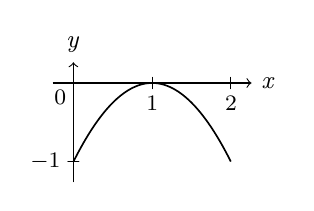
\begin{tikzpicture}
\datavisualization [school book axes,
                    visualize as smooth line,
                    y axis={label},
                    x axis={label} ]

data [format=function] {
			var x : interval [0:2] samples 150;
      func y =  2*\value x -  \value x*\value x - 1 ;
      };
\end{tikzpicture}
 \choice 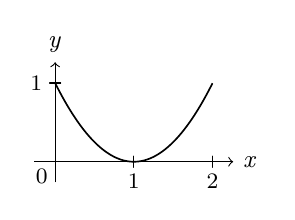
\begin{tikzpicture}
\datavisualization [school book axes,
                    visualize as smooth line,
                    y axis={label},
                    x axis={label} ]

data [format=function] {
			var x : interval [0:2] samples 150;
      func y =   \value x*\value x-2*\value x + 1 ;
      };
\end{tikzpicture}
\choice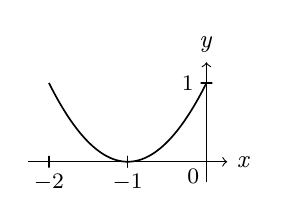
\begin{tikzpicture}
\datavisualization [school book axes,
                    visualize as smooth line,
                    y axis={label},
                    x axis={label} ]

data [format=function] {
			var x : interval [-2:0] samples 150;
      func y =   \value x*\value x+2*\value x + 1 ;
      };
\end{tikzpicture}
 \choice 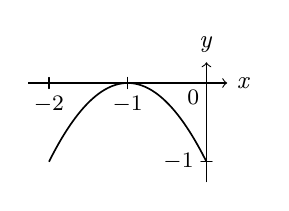
\begin{tikzpicture}
\datavisualization [school book axes,
                    visualize as smooth line,
                    y axis={label},
                    x axis={label} ]

data [format=function] {
			var x : interval [-2:0] samples 150;
      func y =   -\value x*\value x-2*\value x - 1 ;
      };
\end{tikzpicture}

\end{oneparchoices}

\question $\mathlarger{f(x) = x^{2} + 3}$ এবং $\mathlarger{g(x)=\sqrt{x}}$ হয় তবে  $\mathlarger{f( g(x))=?}$  \hfill \textsc{DU:2001-02}

\begin{oneparchoices}
 \choice $\mathlarger{2x+3,\,x<0 }$
\hspace*{.5cm} \choice $\mathlarger{x^2+1}$
 \choice $\mathlarger{3x+9}$
\hspace*{1.7cm}\choice $\mathlarger{x+3,\,x\ge 0}$
\end{oneparchoices}

\question $f(x) = \log_{x+1}(2x+1)$  হলে  $f(x)$ এর ডোমেন কোনটি?  \hfill \textsc{SUST:2016-17}

\begin{oneparchoices}
 \choice $(-\dfrac{1}{2},0)\cup (0,\infty)$
 \choice $x>-1$
 \choice $x\le -\dfrac{1}{2}$
 \choice $(0,\infty)$
 \choice $(-\dfrac{1}{2},-1)\cup (0,\infty)$
\end{oneparchoices}

\question  $\mathlarger{a}$  এর মান কত হলে  $\mathlarger{
 f(x)=\left\{ \begin{array}{cl}
 \frac{x^2}{x} & \textrm{when } x \neq 0\\
a & \textrm{when }x=0
\end
{array}\right.}$ ফাংশনটি অবিচ্ছিন্ন হবে? \hfill \textsc{SUST:2014-15}

\begin{oneparchoices}
 \choice $\mathlarger{-1 }$
 \choice $\mathlarger{1}$
 \choice $\mathlarger{2}$
\choice $\mathlarger{4}$
\choice $\mathlarger{0}$
\end{oneparchoices}

\question $\mathlarger{f(x)= x^2 +1}$ এবং  $\mathlarger{g(x) = \sqrt{2-x}}$ দুইটি  বাস্তব  ফাংশন হলে সংযোজিত  ফাংশন  $gof$ ডোমেন কত?   \hfill \textsc{SUST:2013-14}

\begin{oneparchoices}
 \choice $\mathlarger{(-1,i)}$
 \choice $\mathlarger{[-1,1]}$
 \choice $\mathlarger{(-\infty, \infty)}$
\choice $\mathlarger{(-\infty, 2)}$
\choice $\mathlarger{[2,\infty]}$
\end{oneparchoices}

\question $\mathlarger{f(x-2)= x^2 -2x+1}$ হলে  $\mathlarger{f(-4)}$ এর মান  কত?   \hfill \textsc{SUST:2012-13}

\begin{oneparchoices}
 \choice $\mathlarger{8}$
 \choice $\mathlarger{10}$
 \choice $\mathlarger{12}$
\choice $\mathlarger{16}$
\choice $\mathlarger{32}$
\end{oneparchoices}

\question $\mathlarger{f(x)=\sqrt{x} +\frac{1}{x} -1}$ ফাংশনের ডোমেন -    \hfill \textsc{SUST:2012-13}

\begin{oneparchoices}
 \choice $\mathlarger{(-\infty, 0)}$
 \choice $\mathlarger{(0, \infty)}$
 \choice $\mathlarger{(1, \infty)}$
 \choice $\mathlarger{(-\infty, \infty)}$
 \choice $\mathlarger{(-\infty, 0)\cup (0, \infty)}$
\end{oneparchoices}

\question   ফাংশনের ডোমেন ও রেঞ্জ  $\mathlarger{\{a, b, c, d\}}$  হলে কোনটি 'এক-এক' ফাংশন?\hfill \textsc{SUST:2012-13}

\begin{oneparchoices}
 \choice $f(a)=b, f(b)=c, f(c)=d, f(d)=b$\\
 \choice $f(a)=b, f(b)=c, f(c)=b, f(d)=a$\\
 \choice $f(a)=b, f(b)=c, f(c)=d$\\
 \choice $f(a)=b, f(b)=c, f(c)=d, f(d)=a$\\
 \choice $f(a)=b, f(b)=c, f(c)=d, f(c)=a$
\end{oneparchoices}

\question $\mathlarger{f(x)=0}$ সমীকরণে $f(2+i\sqrt{3}) = 0$ হলে $f(2-i\sqrt{3})$ এর মান কত? \hfill \textsc{SUST:2009-10}

\question $\mathlarger{f(x)=\sqrt{\frac{1-x}{x}}}$ ফাংশনের ডোমেন কত?    \hfill \textsc{SUST:2008-09}

\question $\mathlarger{f(x)=\frac{2x-1}{x-2}}$ ফাংশনের ডোমেন ও রেঞ্জ এবং বিপরীত ফাংশন কোনটি ? \hfill \textsc{SUST:2007-08}

\question $\mathlarger{\phi(x)=\frac{1}{1-x}}$ হলে $\mathlarger{\phi(\phi(\phi(x)))=?}$

\question যদি $\mathlarger{f(x)=x+\frac{1}{x}}$ হয় তবে $\mathlarger{\{f(x) \}^2}$ এর মান কত?

				\begin{oneparchoices}
 \choice $\mathlarger{3+f(x^2)}$
 \choice $\mathlarger{2-f(x^2)}$
 \choice $\mathlarger{2+f(x^2)}$
\choice $\mathlarger{4+f(x^2)}$
\end{oneparchoices}
\begin{center}
\begin{LARGE}
নিচের ফাংশনগুলোর ডোমেন ও রেঞ্জ বের কর -
\end{LARGE}
\end{center}

                                   \question $\mathlarger{f(x)=1-2^{-x}}$

\question $\mathlarger{f(x)=\log_{10} x}$

\question $\mathlarger{f(x)=ln \frac{a+x}{a-x}},\, a>0$

\question $\mathlarger{f(x)= x^2}$

\question $\mathlarger{f(x)= \frac{x}{|x|}}\,$

\question $\mathlarger{f(x)= |x-10|}$

\question $\mathlarger{f(x)= e^{-\frac{|x|}{2}}}\,$

\question $\mathlarger{f(x)= x+|x|}$

\question $\mathlarger{f(x)= \sqrt{2x-1}+\sqrt{3-2x}}$

\question $\mathlarger{f(x)= \frac{1}{\sqrt{|x|-x}}}$

\question $\mathlarger{f(x)= \frac{x^2}{x^4 + 1}}$

\question $\mathlarger{f(x)= \sqrt{3}\sin x + \cos x +4}$

\question $\mathlarger{f(x)= \sqrt{\Bigg( \frac{1}{\sin x} - 1} \Bigg)}$

\question $\mathlarger{f(x)= \frac{\sin ^{-1}(x-3)}{\sqrt{9-x^2}}}$

\question $\mathlarger{f(x)= \Mycomb[7-x]{x-2}}$

\question $\mathlarger{f(x)= \frac{x^2+x+1}{x^2-6x+8}}$

\question $\mathlarger{f(x)= \sqrt{x^2+x-12}}$

\question $\mathlarger{f(x)= \frac{1}{\sqrt{x^2-4x}}}$

\question $\mathlarger{f(x)= \frac{x}{1+x^2}}$

\question $\mathlarger{f(x)= \cos x, \quad (-\frac{\pi}{2} \le x\le \frac{\pi}{2})}$

\question $\mathlarger{f(x)= \sin^{-1}\Bigg( \log_3 \Bigg( \dfrac{x}{3} \Bigg)\Bigg)}$

\end{questions}


\begin{center}
\begin{LARGE}
Exercise-01\\
\end{LARGE}
\begin{large}
 \textbf{ Find the Domain of the following functions:}
\end{large}
\end{center}
\begin{questions}

\question $\mathlarger{f(x)= \sqrt{x^{2}-5}}$

\question $\mathlarger{f(x)= \sin^{-1}(2x-1)}$

\question $\mathlarger{f(x)= \sqrt{\sin x} -\sqrt{16-x^{2}}}$

\question $\mathlarger{f(x)= \dfrac{3}{\sqrt{4-x^{2}}}\log(x^{3}-x)}$

\question $\mathlarger{f(x)= x^{\cos^{-1}x}}$

\question $\mathlarger{f(x)= \dfrac{1}{\log(2-x)} +\sqrt{x+1}}$

\question $\mathlarger{f(x)= \sqrt{1-x} -\sin^{1}\dfrac{2x-1}{3}}$

\question $\mathlarger{f(x)= \dfrac{x^{2}+x+1}{x^{2}+x-1}}$

\question $\mathlarger{f(x)= \ln (2x-x^{2})}$

\question $\mathlarger{f(x)= \sec^{-1}(x^2 +3x+1)}$

\question $\mathlarger{f(x)= \dfrac{x^{2}-2x+5}{x^{2}+2x+5}}$

\question $\mathlarger{f(x)= \dfrac{1}{\sqrt{x^{2}-x}}}$

\question $\mathlarger{f(x)= \cot^{-1}(2x-x^{2})}$

\question $\mathlarger{f(x)= \ln\sin^{-1}\Bigg(x^2 +x+\dfrac{3}{4}\Bigg)}$

\question $\mathlarger{f(x)= \sqrt{\cos 2x} + \sqrt{16-x^2}}$

\question $\mathlarger{f(x)= \log_{7}\log_{5}\log_{3}\log_{2}(2x^3 +5x^2 -14x)}$

\question $\mathlarger{f(x)= \ln(\sqrt{x^2 -5x-24}-x-2)}$

\question $\mathlarger{f(x)= \sqrt{\dfrac{1-5^x}{7^{-x}-7}}}$

\question $\mathlarger{f(x)= \log_{10}\sin(x-3) +\sqrt{16-x^2}}$

\question $\mathlarger{f(x)= \log_{100x}\Bigg(\dfrac{2\log_{10}x+1}{-x}\Bigg)}$

\question $\mathlarger{f(x)= \dfrac{1}{\sqrt{4x^2 -1}}+\ln[x(x^2-1)]}$

\question $\mathlarger{f(x)= \sqrt{\log_{\dfrac{1}{2}}\dfrac{x}{x^{2}-1}}}$

\question $\mathlarger{f(x)= \sqrt{x^2 -|x|} +\dfrac{1}{\sqrt{9-x^2}}}$

\question $\mathlarger{f(x)= \sqrt{(x^{2}-3x-10).\ln^{2}(x-3)}}$

\question $\mathlarger{f(x)= \log_{x}\cos(2\pi x)}$

\question $\mathlarger{f(x)= \dfrac{\sqrt{\cos x -\dfrac{1}{2}}}{\sqrt{6+35x-6x^{2}}}}$

\question $\mathlarger{f(x)= \sqrt{\log_{\frac{1}{3}} (\log_{4}([x]^{2}-5) )}}$

\question $\mathlarger{f(x)= \dfrac{1}{[x]} +\log_{(2\{x\}-5)}(x^{2}-3x+10) + \dfrac{1}{\sqrt{1-|x|}}}$

\question $\mathlarger{f(x)= \log_{x}\sin x }$

\question $\mathlarger{f(x)= \log_{2}\Bigg[-\log_{\dfrac{1}{2}} \Bigg(1+\dfrac{1}{\sin \Bigg(\dfrac{x^{\circ}}{100}\Bigg)} \Bigg] +\sqrt{\log_{10}(\log_{10}x) -\log_{10}(4-\log_{10}x) -\log_{10}3}}$

\question $\mathlarger{f(x)= \dfrac{1}{[x]} + \log_{1-\{x\}} (x^2 -3x +10) +\dfrac{1}{\sqrt{2-|x|}} +\dfrac{1}{\sqrt{\sec(\sin x)}}}$

\question $\mathlarger{f(x)= \sqrt{(5x-6-x^2)[\{\ln\{x\}\}]} +\sqrt{(7x-5-2x^{2})} +\Bigg[\ln\Bigg(\dfrac{7}{2}-x\Bigg) \Bigg]^{-1} }$

\end{questions}
\begin{center}
\begin{large}
 \textbf{ Find the Domain and the Range of the following functions:}
\end{large}
\begin{LARGE}
Excercise-02
\end{LARGE}
\end{center}

\begin{questions}
\question $\mathlarger{f(x)= \log_{\sqrt{5}} \Big(\sqrt{2}(\sin x -\cos x) +3 \Big ) }$

\question $\mathlarger{f(x)= \dfrac{2x}{1+x^{2}}}$

\question $\mathlarger{f(x)= \dfrac{x^2 -3x +2}{x^2 +x -6}}$

\question $\mathlarger{f(x)= \dfrac{x}{1+|x|}}$

\question $\mathlarger{f(x)= \sqrt{2-x} +\sqrt{1+x}}$

\question $\mathlarger{f(x)= \log_{(cosec x -1)} (2-[\sin x]  -[\sin x]^{2})}$

\question $\mathlarger{f(x)= \dfrac{\sqrt{x+4} -3}{x-5}}$

\question $\mathlarger{ f(x)=\sqrt{\sin\left(\log_{e}\left(\dfrac{x^2+e}{x^2+1}\right)\right)}+\sqrt{\cos\left(\log_{e}\left(\dfrac{x^2+e}{x^2+1}\right)\right)}}$
%Here, the questions begin

			\question $f(x)=\mathlarger{\sqrt{\log_{10}\left(\dfrac{1-2x}{x+3}\right)} }$
\end{questions}
\begin{center}
\begin{LARGE}
Exercise-01
Answers:
\end{LARGE}
\end{center}
\begin{questions}

\question $\mathlarger{(-\infty, -\sqrt{5}]\cup [ \sqrt{5}, \infty)}$

\question $\mathlarger{x\in [0,1]}$

\question $\mathlarger{D_{f} = \{x: x\in [2n\pi, (2n+1)\pi], n\in \mathbb{Z} \}\cap [-4,4] = [-4,-\pi]\cup [0,\pi] }$

\question $\mathlarger{D_{f}=\{(-1,0)\cup(1,\infty)\}\cap (-2,2) =(-1,0)\cup (1,2)}$

\question $\mathlarger{(0,1]}$

\question $\mathlarger{[-1,1)\cup (1,2)}$

\question $\mathlarger{[-1,1]}$

\question $\mathlarger{R_{f}=(-\infty, -\dfrac{3}{5}\Bigg] \cup (1,\infty)}$

\question $\mathlarger{D_{f} = (0,1],\quad R_{f} = (-\infty, 0]}$

\question $\mathlarger{D_{f} = \Bigg[-\dfrac{5}{4}, -1 \Bigg] \cup [1,\infty),\quad R_{f} = \Bigg[ 0,\dfrac{\pi}{2}\Bigg) \cup \Bigg[\sec^{-1}\Bigg(-\dfrac{5}{4}\Bigg),\pi\Bigg]}$

\question $\mathlarger{R_{f}= \Bigg[\dfrac{3-\sqrt{5}}{2}, \dfrac{3+\sqrt{5}}{2} \Bigg]}$

\question $\mathlarger{D_{f} = \mathbb{R}-[0,1],\quad R_{f} = (0,\infty)}$

\question $\mathlarger{D_{f} = \mathbb{R},\quad R_{f} = \Bigg[\dfrac{\pi}{4}, \pi\Bigg]}$

\question $\mathlarger{D_{f} = \Bigg[ \dfrac{-2-\sqrt{5}}{4}, \dfrac{-2+\sqrt{5}}{4}\Bigg],\quad R_{f} = \Bigg[\ln\dfrac{\pi}{6}, \ln\dfrac{\pi}{2}  \Bigg]}$

\question $\mathlarger{\Bigg[-\dfrac{5\pi}{4}, -\dfrac{3\pi}{4} \Bigg]\cup \Bigg[-\dfrac{\pi}{4}, \dfrac{\pi}{4} \Bigg]\cup \Bigg[\dfrac{3\pi}{4}, \dfrac{5\pi}{4} \Bigg]}$

\question $\mathlarger{\Bigg(-4,-\dfrac{1}{2}\Bigg)\cup (2,\infty)}$

\question $\mathlarger{(-\infty, 3]}$

\question $\mathlarger{(-\infty, -1)\cup [0,\infty)}$

\question $\mathlarger{(3-2\pi<x<3-\pi)\cup (3<x\le 4)}$

\question $\mathlarger{\Bigg( 0,\dfrac{1}{100}\Bigg)\cup \Bigg(\dfrac{1}{100}, \dfrac{1}{\sqrt{10}}\Bigg)}$

\question $\mathlarger{\Bigg(-1<x<-\dfrac{1}{2}\Bigg)\cup(x>1)}$

\question $\mathlarger{\Bigg[ \dfrac{1-\sqrt{5}}{2}, 0\Bigg)\cup \Bigg[ \dfrac{1+\sqrt{5}}{2},\infty\Bigg)}$

\question $\mathlarger{(-3,-1)\cup \{0\}\cup [1,3)}$

\question $\mathlarger{\{4\}\cup [5,\infty)}$

\question $\mathlarger{\Bigg(0,\dfrac{1}{4}\Bigg)\cup \Bigg(\dfrac{3}{4}, 1\Bigg)\cup\{x:x \in \mathbb{N}, x\ge 2\}}$

\question $\mathlarger{\Bigg(-\dfrac{1}{6},\dfrac{\pi}{3}\Bigg]\cup \Bigg[\dfrac{5\pi}{3},6\Bigg)}$

\question $\mathlarger{[-3,-2)\cup [3,4)}$

\question $\mathlarger{\phi}$

\question $\mathlarger{2n\pi <x<(2n+1)\pi}$ but $\mathlarger{x\neq 1}$ where $\mathlarger{n}$ is non-negative integer.

                                                                                                              \question $\mathlarger{\{x|1000\le x < 10000\}}$

\question $\mathlarger{(-2,-1)\cup (-1,0)\cup(1,2)}$

\question $\mathlarger{(1,2)\cup \Bigg(2,\dfrac{5}{2}\Bigg)}$

\end{questions}
\begin{center}
\begin{LARGE}
Exercise-02
Answers:
\end{LARGE}
\end{center}
\begin{questions}

\question $\mathlarger{D_{f} = x\in \mathbb{R},\quad R_{f} = [0,2]}$

\question $\mathlarger{D_{f} = \mathbb{R},\quad R_{f} = [-1,1]}$

\question $\mathlarger{D_{f} = \{x|x\in \mathbb{R}; x\neq -3; x\neq 2 \},\quad R_{f} = \{f(x)|f(x)\in \mathbb{R},\, f(x)\neq \dfrac{1}{5};\,f(x)\neq 1\} }$

\question $\mathlarger{D_{f} = \mathbb{R},\quad R_{f} = (-1,1)}$

\question $\mathlarger{D_{f} = -1\le x \le 2,\quad R_{f} = [\sqrt{3},\sqrt{6}]}$

\question $\mathlarger{D_{f} = x\in \Bigg(2n\pi, (2n+1)\pi\Bigg)} - \Bigg\{ 2n\pi + \dfrac{\pi}{6}, 2n\pi + \dfrac{\pi}{2}, 2n\pi + \dfrac{5\pi}{6}, n\in \mathbb{Z} \Bigg\}$ and\\ $\mathlarger{R_{f} = \log_{a}2;\, a\in (0,\infty)-\{1\} = \{-\infty, \infty\}-\{0\}}$

\question $\mathlarger{D_{f} =[-4, \infty) - \{5\},\quad R_{f} = \Bigg(0,\dfrac{1}{6}\Bigg) \cup \Bigg(\dfrac{1}{6}, \dfrac{1}{3}\Bigg]}$

\end{questions}
\end{document}






